\section{Theory}
\subsection{An Optical Cavity}

An optical cavity is generally comprised of two highly reflective optical resonators. It is used for trapping any amount of light for an extended period of time, thus increasing the effective cross section of a given interaction between some object and the field inside the cavity. 

Another attribute of the optical cavity is that it gives rise to so-called eigenstates related to the length of the cavity\cite{Eichhorn}. As the cavity does not expand infinitely, the allowed modes inside the cavity are limited to ones which fulfill the identity \cite{Pedrotti}
\begin{equation}
    2 d \cos \theta = m \lambda.
\end{equation}
Here \emph{d} is the length of the cavity, $\theta$ is the incidence angle of the light coupling into the cavity, $\lambda$ is the wavelength of the light and $m = 1,2,3,...$ is a positive integer describing the order of the mode. For the rest of this thesis it will be assumed that the laser couples into the cavity at normal incidence, meaning that $\theta = 0^{\circ}$ and thus $\cos \theta = 1$.

\subsubsection{The Fundamental Mode: A Gaussian Beam in the Large Waist Approximation}

In order to describe the allowed modes within an optical cavity, it is first assumed that a single-mode field is linearly polarized. We then consider solutions to the wave equation
\begin{equation}
    \nabla^2 \vec{E} = \frac{1}{c^2} \frac{\partial^2 \vec{E}}{\partial t^2},
\end{equation}
given as
\begin{equation}
    \vec{E} = E_0 (x,y,z) \vec{\epsilon} e^{i k z}. 
\end{equation}
Here $E_0(x,y,z)$ describes the electric field amplitude, $\vec{\epsilon}$ is denoted the polarization vector and $k=2 \pi / \lambda$ is the angular wave number of the field propagating along the z-axis. It is assumed that the electric field has a Gaussian transverse distribution\footnote{When this is the case, the laser is said to operate in the lowest possible mode denoted $TEM_{00}$. This implies the assumption of ideal lasing conditions.}.

This is almost the simplest description of the propagating field, however, as the spacial dependence of the field amplitude still might cause problems, we consider the range in which this can be neglected. 

It can be shown from the derivation of the Gaussian distribution that the waist of the beam $w(z)$, which depends on the spacial coordinate in the direction of propagation, can be described as \cite{Eichhorn}
\begin{equation}
    w(z) = w_0 \sqrt{1 + \left(\frac{z}{z_R}\right)^2},
    \label{eq:gaussian beam waist}
\end{equation}
where $z$ is the distance from focus, $w_0$ is the beam waist at focus and $z_R$ is the so-called \emph{Rayleigh range}. The Rayleigh range describes the range in which the beam diverges slowly, whereas after this has been surpassed, the beam will begin to diverge more rapidly. By quick inspection of eq. (\ref{eq:gaussian beam waist}) it is seen that
\begin{equation}
    w(z) = 
    \begin{cases}
        w_0, & \mbox{for } z=0 \\
        w_0\sqrt{2}, & \mbox{for } z=z_R,
    \end{cases}
\end{equation}
which shows that the beam waist diverges no more than by a factor of $\sqrt{2}$ from the optimal case, for $0\leq z \leq z_R$. Considering the case where $z \neq 0$ but however much smaller than the Rayleigh range $z_R$, we can further inspect eq. (\ref{eq:gaussian beam waist}) and find that this leads to negligible changes in the waist of the beam. Specifically, it can fairly easily be seen that
\begin{equation}
    \left(\frac{z}{z_R}\right)^2 \approx 0, \: \text{  for } z << z_R
\end{equation}
which in turn leads to 
\begin{equation}
    w(z) \approx w_0.
\end{equation}

The Rayleigh range can be written as \cite{Pedrotti}
\begin{equation}
    z_R = \frac{\pi w_0^2}{\lambda},
    \label{eq:Rayleigh range}
\end{equation}
which, through the exponential dependence on $w_0$, shows that a large beam waist will result in a long Rayleigh range. As an example, consider a beam of waist $w_0 = 200 \mu m$ and wavelength $\lambda = 950 nm$. This would result in a Rayleigh range of $z_R=13.23 cm$. 

Finally we can conclude, that any optical cavity, for which the total distance travelled inside the cavity\footnote{For any optical cavity the incident light will travel a distance inside the cavity according to, not only the length of the cavity, but also the amount of round trips the light makes when confined inside the cavity.}, is significantly shorter than the Rayleigh range of the incident beam, the spacial dependence of the field amplitude inside the cavity is negligible, and the fundamental mode can be described simply by a linearly polarized plane wave
\begin{equation}
    \vec{E} = E_0 \vec{\epsilon} e^{ikz}.
\end{equation}
This is often referred to as the \emph{large waist approximation} of a Gaussian beam, due to the dependence on $w_0$ of eq. (\ref{eq:Rayleigh range}).

\subsubsection{The Fabry-Perot Interferometer}

\begin{figure}
    \centering
    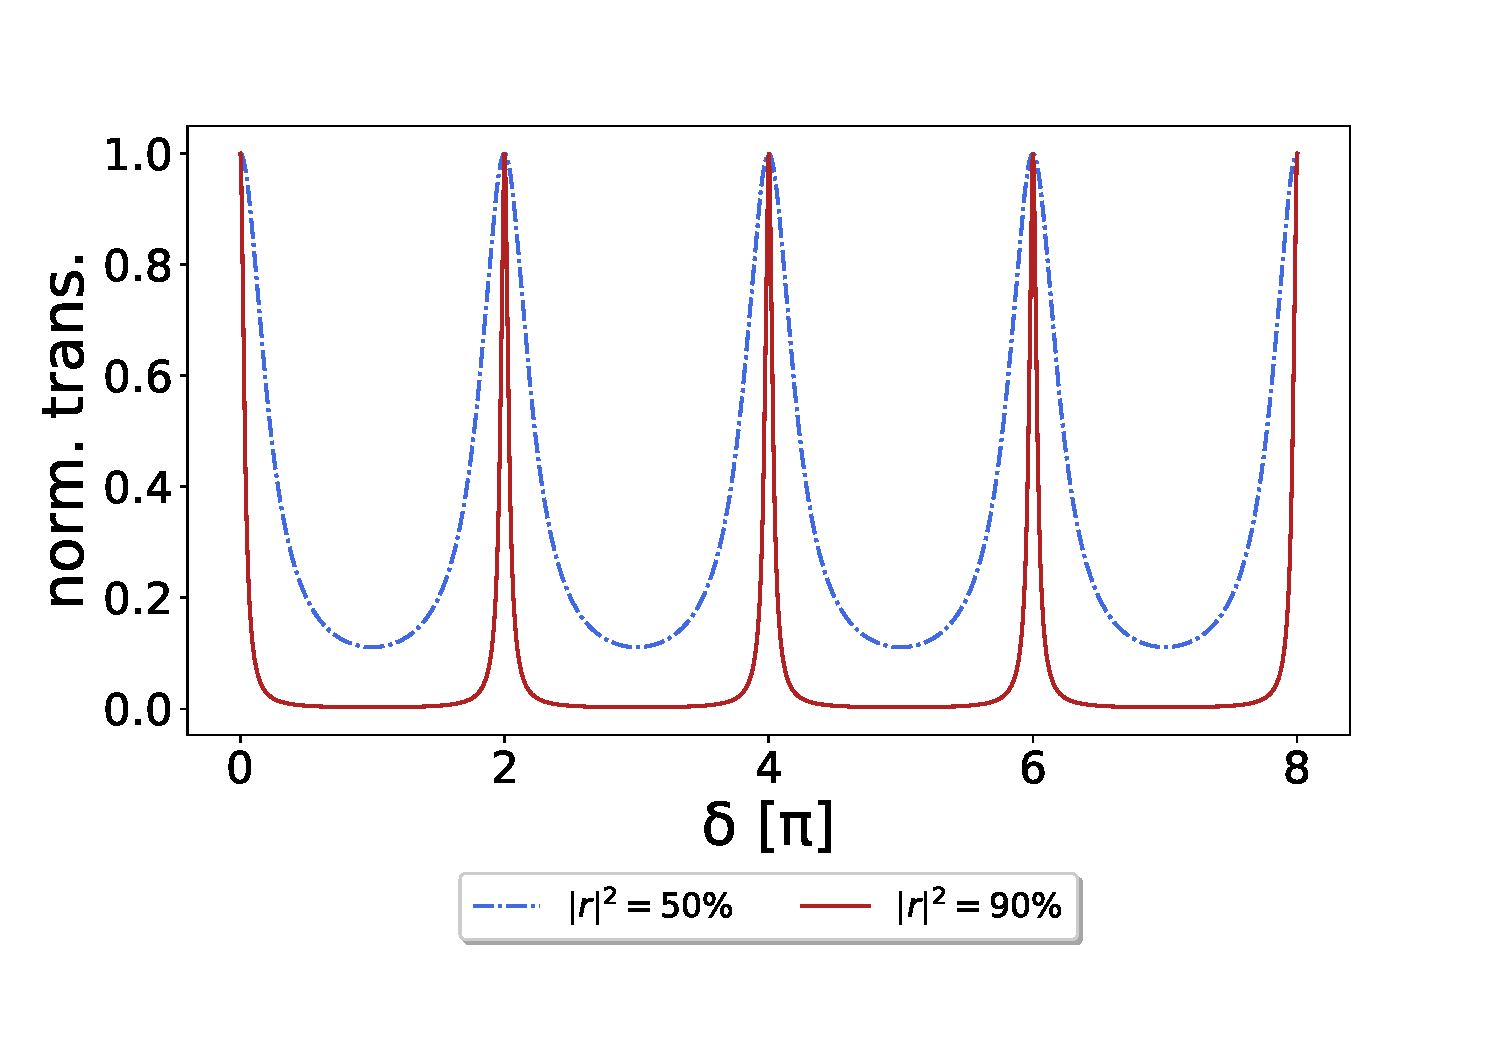
\includegraphics[width=0.6\textwidth]{figures/fabry_perot_high_and_low_finesse.pdf}
    \caption{Comparison of an arbitrary Fabry-Perot cavity of high and low finesse, respectively. The high finesse cavity and a reflectivity of $|r|^2 = 0.90$, while for the low finesse cavity $|r|^2 = 0.30$.}
\end{figure}